% VUT FIT MITAI
% MSZ 2021/2022
% Author: Vladimir Dusek
% Login: xdusek27

%%%%%%%%%%%%%%%%%%%%%%%%%%%%%%%%%%%%%%%%%%%%%%%%%%%%%%%%%%%%%%%%%%%%%%%%%%%%%%%%

% Path to figures
\graphicspath{{tin/slozitost/figures}}

%%%%%%%%%%%%%%%%%%%%%%%%%%%%%%%%%%%%%%%%%%%%%%%%%%%%%%%%%%%%%%%%%%%%%%%%%%%%%%%%

\chapter{TIN~--~Časová a paměťová složitost (třídy složitosti, úplnost, SAT problém).}

%%%%%%%%%%%%%%%%%%%%%%%%%%%%%%%%%%%%%%%%%%%%%%%%%%%%%%%%%%%%%%%%%%%%%%%%%%%%%%%%

\section{Zdroje}

\begin{compactitem}
    \item \path{tin_2021_merged.pdf}
    \item \path{TIN_2020-12-01.mp4}
    \item \path{TIN_2020-12-04_demo.mp4}
    \item \path{TIN_2020-12-08.mp4}
    \item \path{TIN_2020-12-11_demo.mp4}
\end{compactitem}

%%%%%%%%%%%%%%%%%%%%%%%%%%%%%%%%%%%%%%%%%%%%%%%%%%%%%%%%%%%%%%%%%%%%%%%%%%%%%%%%

\section{Úvod a kontext}

% složitost problému vs složitost algoritmu ?

% Co je to NP-úplnost, co je obecně úplnost a těžkost.

% Chtěl slyšet příklad nějakého NP-úplného problému. Když jsem řekl SAT, tak chtěl definovat, co je to SAT problém.

\begin{compactitem}
    \item Časová složitost -- počet kroků (přechodů) TS provedený od počátku do konce výpočtu.

    \item Prostorová (paměťová) složitost -- počet buněk pásky TS požadovaný pro daný výpočet.

    \item Je-li časová složitost výpočtu prováděného TS rovna $n$, pak prostorová složitost tohoto výpočtu není větší než $n + 1$. \begin{compactitem}
        \item Tvrzení je jednoduchou implikací plynoucí z definice časové a prostorové složitosti.
    \end{compactitem}

    \item Při popisu složitosti algoritmů (výpočtů TS), chceme často vyloučit vliv aditivních a multiplikativních konstant: \begin{compactitem}
        \item Různé aditivní a multiplikativní konstanty vzniknou velmi snadno \uv{drobnými} úpravami uvažovaných algoritmů.
        \item Primárně nás zajímá, jak složitost roste v závislosti na délce vstupu. Zejméne pro dlouhé vstupy.
    \end{compactitem}

    \item Různé případy při analýze složitosti: \begin{compactitem}
        \item analýza složitosti nejhoršího případu,
        \item analýza složitosti nejlepšího případu,
        \item analýza složitosti průměrného případu,
        \item amortizovaná analýza -- Studuje posloupnost operací jako celek. Tato technika umožňuje, na rozdíl od klasického přístupu mnohem přesnější určení časové složitosti algoritmu.
    \end{compactitem}

\end{compactitem}

%%%%%%%%%%%%%%%%%%%%%%%%%%%%%%%%%%%%%%%%%%%%%%%%%%%%%%%%%%%%%%%%%%%%%%%%%%%%%%%%

\section{Asymptotická složitost}

\begin{compactitem}
    \item Složitost algoritmů, resp. turingových strojů.

    \item Asymptotická složitost -- neřešíme aditivní a multiplikativní konstanty a bereme v potaz pouze nejvyšší polynom.

    \item Nechť $\mathcal{F}$ je množina funkcí $f : \mathbb{N} \rightarrow \mathbb{N}$. Pro danou funkci $f \in \mathcal{F}$ definujeme množiny funkcí $\mathcal{O}(f(n))$, $\Omega(f(n))$ a $\Theta(f(n))$ následovně: \begin{compactitem}

        \item \textbf{Asymptotické horní omezení} funkce $f(n)$ je množina
        $$ \mathcal{O}(f(n)) = \{ g(n) \in \mathcal{F} ~|~ \exists c \in \mathbb{R}^{+} ~\exists n_0 \in \mathbb{N} ~\forall n \in \mathbb{N} : n \geq n_0 \Rightarrow $$
        $$ \Rightarrow 0 \leq g(n) \leq c \cdot f(n) \} $$

        \item \textbf{Asymptotické dolní omezení} funkce $f(n)$ je množina
        $$ \Omega(f(n)) = \{ g(n) \in \mathcal{F} ~|~ \exists c \in \mathbb{R}^{+} ~\exists n_0 \in \mathbb{N} ~\forall n \in \mathbb{N} : n \geq n_0 \Rightarrow $$
        $$ \Rightarrow 0 \leq c \cdot f(n) \leq g(n) \} $$

        \item \textbf{Asymptotické oboustranné omezení} funkce $f(n)$ je množina
        $$ \Theta(f(n)) = \{ g(n) \in \mathcal{F} ~|~ \exists c_1, c_2 \in \mathbb{R}^{+} ~\exists n_0 \in \mathbb{N} ~\forall n \in \mathbb{N} : n \geq n_0 \Rightarrow $$
        $$ \Rightarrow 0 \leq c_1 \cdot f(n) \leq g(n) \leq c_2 \cdot f(n) \} $$

    \end{compactitem}
\end{compactitem}

\begin{figure}[H]
    \centering
    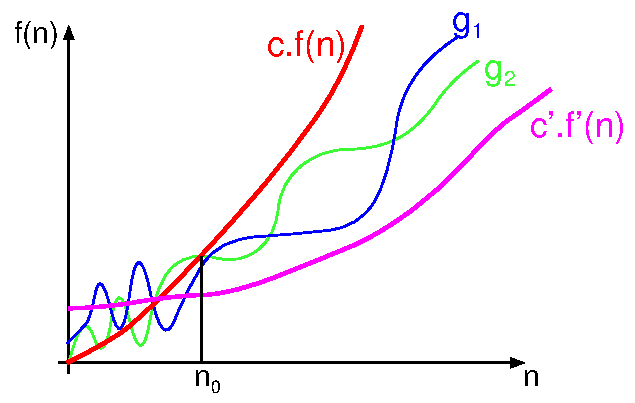
\includegraphics[width=0.75\linewidth]{complexity.pdf}
    \caption{Asymptotická složitost.}
\end{figure}

%%%%%%%%%%%%%%%%%%%%%%%%%%%%%%%%%%%%%%%%%%%%%%%%%%%%%%%%%%%%%%%%%%%%%%%%%%%%%%%%

\section{Třídy složitosti}

\begin{compactitem}
    \item Složitosti problémů.

    \item Třídy složitosti zavádíme jako prostředek ke kategorizaci (vytvoření hierarchie) problémů dle jejich složitosti, tedy dle toho, jak dalece efektivní algoritmy můžeme navrhnout pro jejich rozhodování.

    \item Mějme dány funkce $t, s : \mathbb{N} \rightarrow \mathbb{N}$ a nechť $T_M$, resp. $S_M$, značí časovou, resp. prostorovou, složitost TS $M$. Definujeme následující časové a prostorové třídy složitosti deterministických a nedeterministických TS:

    $$DTime[ t(n) ] = \{ L ~|~ \exists k \text{-páskový DTS } M : L = L(M) ~\land~ T_M \in \mathcal{O}(t(n)) \}$$

    $$NTime[ t(n) ] = \{ L ~|~ \exists k \text{-páskový NTS } M : L = L(M) ~\land~ T_M \in \mathcal{O}(t(n)) \}$$

    $$DSpace[ s(n) ] = \{ L ~|~ \exists k \text{-páskový DTS } M : L = L(M) ~\land~ S_M \in \mathcal{O}(s(n)) \}$$

    $$NSpace[ s(n) ] = \{ L ~|~ \exists k \text{-páskový NTS } M : L = L(M) ~\land~ S_M \in \mathcal{O}(s(n)) \}$$

    \item Definici tříd složitosti pak přímočaře zobecňujeme tak, aby mohly být založeny na množině funkcí, nejen na jedné konkrétní funkci.
\end{compactitem}

\subsection{Konkrétní třídy složitosti}

\paragraph*{Deterministický/nedeterministický polynomiální čas} Pro všechny třídy platí, že $n$ je délka vstupu a $k$ je konstanta. $$ \mathbf{P} = \bigcup_{k=0}^{\infty} DTime(n^k) ~~~~~ \equiv^? ~~~~~ \mathbf{NP} = \bigcup_{k=0}^{\infty} NTime(n^k) $$

\paragraph*{Deterministický/nedeterministický polynomiální prostor} $$ \mathbf{PSPACE} = \bigcup_{k=0}^{\infty} DSpace(n^k) ~~~~~ \equiv ~~~~~ \mathbf{NPSPACE} = \bigcup_{k=0}^{\infty} NSpace(n^k) $$

\paragraph*{Deterministický/nedeterministický logaritmický prostor} $$ \mathbf{LOGSPACE} = \bigcup_{k=0}^{\infty} DSpace(k \cdot \log(n)) ~~~~~ \equiv^? ~~~~~ \mathbf{NLOGSPACE} = \bigcup_{k=0}^{\infty} NSpace(k \cdot \log(n)) $$

\paragraph*{Deterministický/nedeterministický exponenciální čas} $$ \mathbf{EXP} = \bigcup_{k=0}^{\infty} DTime(2^{n^k}) ~~~~~ \equiv^? ~~~~~ \mathbf{NEXP} = \bigcup_{k=0}^{\infty} NTime(2^{n^k}) $$

\paragraph*{Deterministický/nedeterministický exponenciální prostor} $$ \mathbf{EXPSPACE} = \bigcup_{k=0}^{\infty} DSpace(2^{n^k}) ~~~~~ \equiv ~~~~~ \mathbf{NEXPSPACE} = \bigcup_{k=0}^{\infty} NSpace(2^{n^k}) $$

\medskip \noindent Neformálně: třídy složitosti jsou množiny problémů, pro které existuje k-páskový TS takový, že je dokáže řešit v nějaké časové/prostorové složitosti.

\subsection{Příklady}

\paragraph*{1) Dokažte, že $2n + 5 \in \mathcal{O}(n) $} \begin{compactitem}
    \item Z definice $\mathcal{O}(n)$: $$ c \cdot n \geq 2n + 5 ~\text{pro}~ \forall n \geq n_0 $$

    \item Nerovnice platí pro $c = 3$ a $n_0 = 5$.
\end{compactitem}

\paragraph*{2) Dokažte, že $ n^2 \not\in \mathcal{O}(n) $} \begin{compactitem}
    \item Dokážeme sporem.

    \item Z definice $\mathcal{O}(n)$, musí existovat $c$ a $n_0$ takové, že $$ c \cdot n \geq n^2 ~\text{pro}~ \forall n \geq n_0 $$

    \item Nechť $m \geq n_0$, pak platí: $$ m^2 > c \cdot m ~\Rightarrow~ m > c $$

    \item Potom: $$ m \geq n_0 ~\land~ m > c $$

    \item A tedy $$ m = max(c, n_0) + 1$$

    \item Dosadíme zpět $m$: $$ max(c, n_0) + 1 \geq n_0 ~\land~ max(c, n_0) + 1 > c $$

    \item Což je spor.
\end{compactitem}

\paragraph*{3) Dokažte, že $ L = \{ w ~|~ w \in \Sigma^* \land w=w^R \} $ patří do $ DTime(n) $} \begin{compactitem}
    \item Dokáže se, sestrojením algoritmu.
    \item Využijeme 2 páskový TS, postup: \begin{compactenum}
        \item TS se přesune na konec první pásky -- $\mathcal{O}(n)$.
        \item TS kopíruje obsah první pásky od konce na druhou pásku -- $\mathcal{O}(n)$.
        \item TS se přesune na začátek druhé pásky -- $\mathcal{O}(n)$.
        \item TS postupně znak po znaku porovnává obsah obou pásek -- $\mathcal{O}(n)$.
    \end{compactenum}
    \item Celkově $4 \mathcal{O}(n) = \mathcal{O}(n)$ a tady $L \in DTime(n)$.
\end{compactitem}

%%%%%%%%%%%%%%%%%%%%%%%%%%%%%%%%%%%%%%%%%%%%%%%%%%%%%%%%%%%%%%%%%%%%%%%%%%%%%%%%

\section{Vlastnosti tříd složitosti}

\paragraph*{Vícepáskový a jednopáskový TS} \begin{compactitem}
    \item Je-li jazyk $L$ přijímán nějakým $k$-páskovým DTS $M_k$ v čase $t(n)$, pak je také přijímán nějakým 1-páskovým DTS $M_1$ v čase $\mathcal{O}(t(n)^2)$. \begin{compactitem}
        \item Více pásek nepřináší nic z pohledu vyčíslitelnosti.
        \item Z pohledu časové složitosti přináší více pásek polynomiální zrychlení (resp. kvadratické).
    \end{compactitem}
\end{compactitem}

\paragraph*{Deterministický a nedeterministický TS} \begin{compactitem}

    \item Je-li jazyk $L$ přijímán nějakým NTS $M_n$ v čase $t(n)$, pak je také přijímán nějakým DTS $M_d$ v čase $2^{\mathcal{O}(t(n))}$. \begin{compactitem}
        \item Nedeterminismus nepřináší nic z pohledu vyčíslitelnosti.
        \item Z pohledu časové složitosti, lze NTS implementovat deterministickým TS, ale za cenu exponenciálního nárůstu času.
    \end{compactitem}

    \item (Savitchův teorém) $NSpace[s(n)] \subseteq DSpace[s^2 (n)]$ pro každou prostorově zkonstruovatelnou funkci $s(n) \geq \log{n}$.\begin{compactitem}
        \item Z pohledu prostorové složitosti, lze NTS implementovat deterministickým TS, ale za cenu kvadratického nárůstu prostoru.
        \item Proto $\mathbf{PSPACE} \equiv \mathbf{NPSPACE}$.
    \end{compactitem}
\end{compactitem}

\paragraph*{Vztah prostoru a času} Intuitivně můžeme říci, že zatímco prostor může růste relativně pomalu, čas může růst výrazně rychleji, neboť můžeme opakovaně procházet týmiž buňkami pásky -- opačně tomu být zřejmě nemůže (nemá smysl mít nevyužitý prostor).

\paragraph*{Uzavřenost vůči doplňku} Doplňkem třídy rozumíme třídu jazyků, které jsou doplňkem jazyků dané třídy. Tedy označíme-li doplněk třídy $\mathcal{C}$ jako $co\text{-}\mathcal{C}$, pak $L \in \mathcal{C} \Leftrightarrow \bar{L} \in co\text{-}\mathcal{C}$. U rozhodování problémů toto znamená rozhodování komplementárního problému (prázdnost $\times$ neprázdnost apod). \begin{compactitem}
    \item Prostorové třídy jsou obvykle uzavřeny vůči doplňku.
    \item Pro časové třídy je situace jiná: \begin{compactitem}
        \item Některé třídy jako $\mathbf{P}$ či $\mathbf{EXP}$ jsou uzavřeny vůči doplňku.
        \item U jiných významných tříd zůstává otázka uzavřenosti vůči doplňku otevřená. Proto má smysl hovořit např. i o třídách jako $\mathbf{co\text{-}NP}$, $\mathbf{co\text{-}NEXP}$, \dots
    \end{compactitem}
\end{compactitem}

\begin{figure}[H]
    \centering
    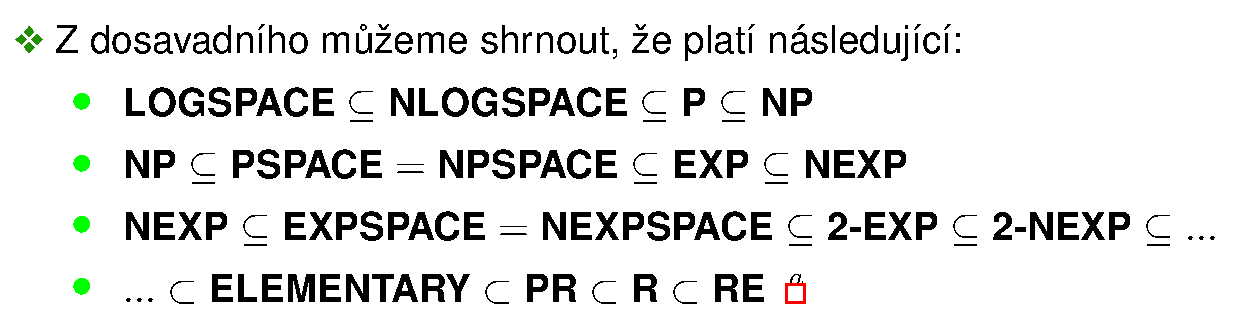
\includegraphics[width=0.9\linewidth]{complexity_class_hierarchy.pdf}
    \caption{Hierarchie složitostních tříd. $\mathbf{ELEMENTARY}$ je \uv{věž} exponenciál jejiž výška je závislá na délce vstupu. $\mathbf{PR}$ jsou primitivně rekurizvní, $\mathbf{R}$ rekurizvní a $\mathbf{RE}$ rekurzivně vyčíslitelné třídy.}
\end{figure}

\begin{figure}[H]
    \centering
    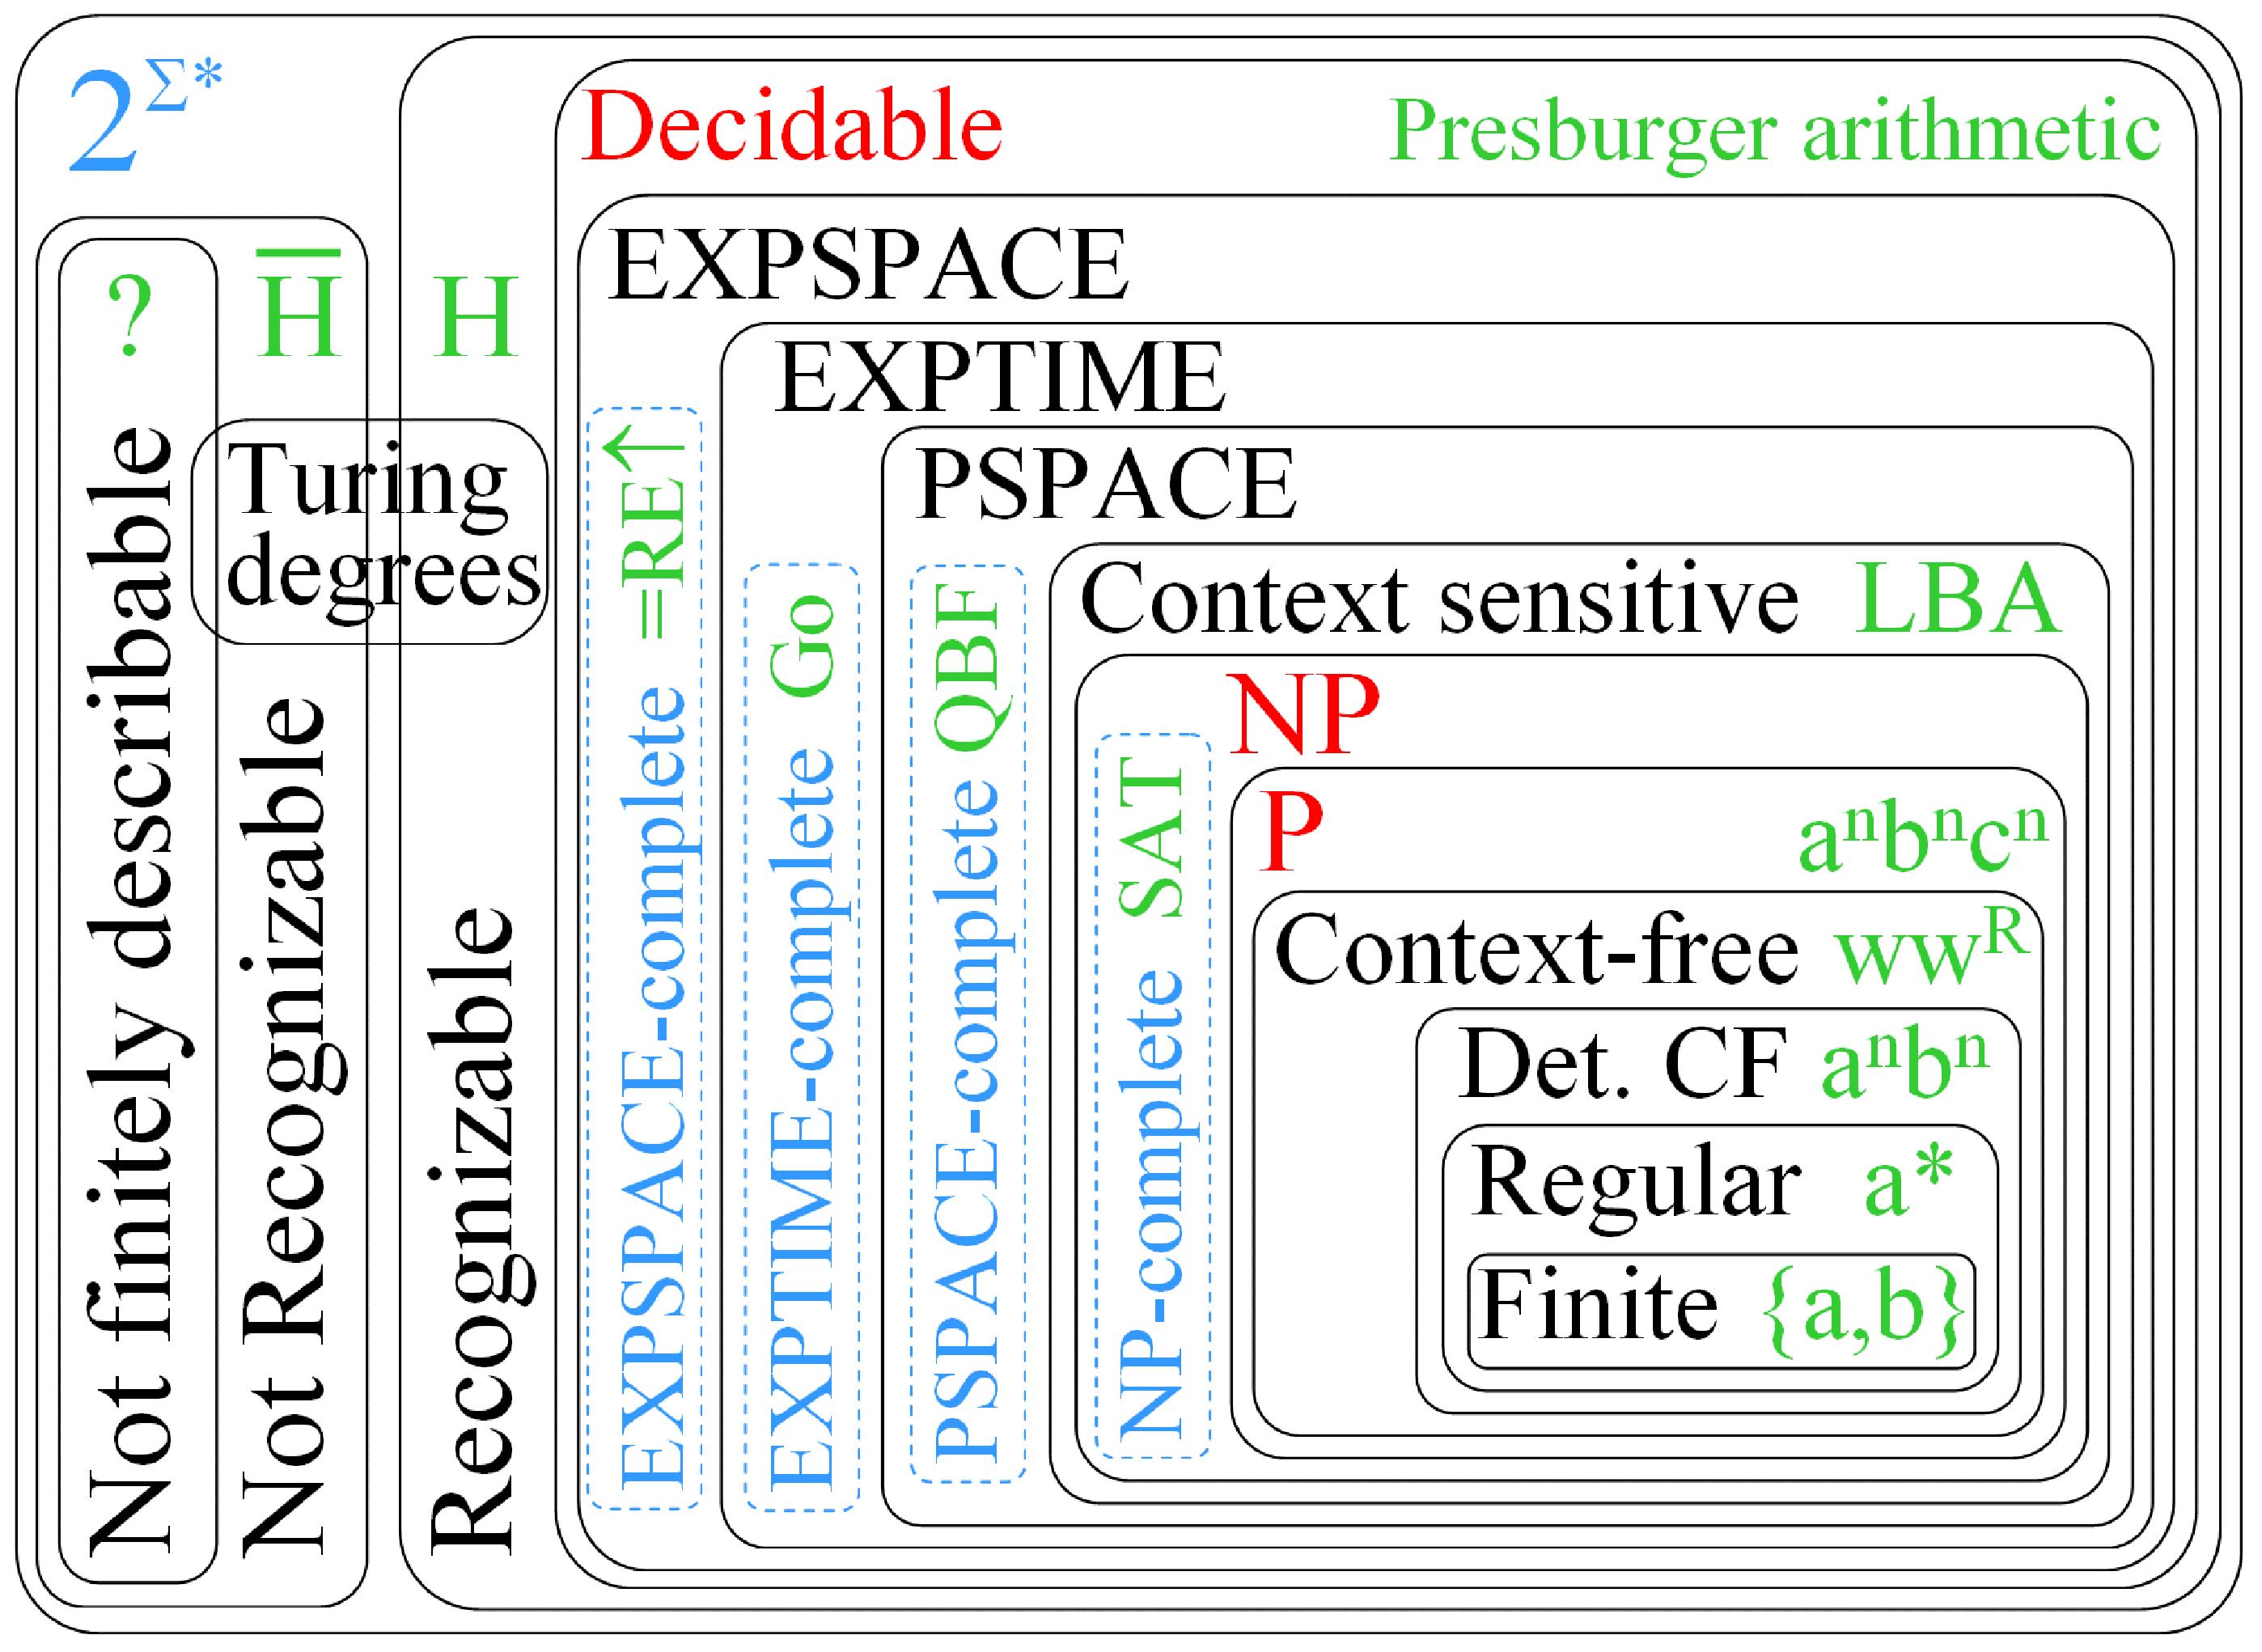
\includegraphics[width=0.9\linewidth]{chomsky_extended.pdf}
    \caption{Rozšířená Chomského hierarchie.}
\end{figure}

%%%%%%%%%%%%%%%%%%%%%%%%%%%%%%%%%%%%%%%%%%%%%%%%%%%%%%%%%%%%%%%%%%%%%%%%%%%%%%%%

\section{Redukce, úplnost, těžkost}

\begin{compactitem}
    \item Až doposud jsme třídy používali jako horní omezení složitosti problémů. Všimněme si nyní omezení dolního -- to zavedeme pomocí redukovatelnosti třídy problémů na daný problém.
\end{compactitem}

\paragraph*{Redukovatelnost} Nechť $\mathcal{R}$ je třída funkcí. Jazyk $L_1 \subseteq \Sigma_1^*$ je $\mathcal{R}$-redukovatelný (přesněji $\mathcal{R}$ \textit{many-to-one reducible}) na jazyk $L_2 \subseteq \Sigma_2^*$, což zapisujeme $L_1 \leq_{\mathcal{R}}^m L_2$, jestliže existuje funkce $f \in \mathcal{R}$ taková, že $\forall w \in \Sigma_1^* : w \in L_1 \Leftrightarrow f(w) \in L_2$. \begin{compactitem}
    \item Jazyk je redukovatelný na jiný jazyk jesliže existuje funkce, která tuto redukci realizuje.
\end{compactitem}

\paragraph*{Těžkost} Nechť $\mathcal{R}$ je třída funkcí a $\mathcal{C}$ třída jazyků. Jazyk $L_0$ je $\mathcal{C}$-těžký ($\mathcal{C}$\textit{-hard}) vzhledem k $\mathcal{R}$ redukovatelnosti, jestliže $\forall L \in \mathcal{C} : L \leq_\mathcal{R}^m L_0$. \begin{compactitem}
    \item Jazyk je $\mathcal{C}$-těžký, jesliže lze všechny jazyky z třídy $\mathcal{C}$ na něj $\mathcal{R}$-redukovat.
\end{compactitem}

\paragraph*{Úplnost} Nechť $\mathcal{R}$ je třída funkcí a $\mathcal{C}$ třída jazyků. Jazyk $L_0$ nazveme $\mathcal{C}$-úplný ($\mathcal{C}$\textit{-complete}) vzhledem k $\mathcal{R}$ redukovatelnosti, jestliže $L_0 \in \mathcal{C}$ a $L_0$ je $\mathcal{C}$-těžký ($\mathcal{C}$\textit{-hard}) vzhledem k $\mathcal{R}$ redukovatelnosti. \begin{compactitem}
    \item Jazyk je $\mathcal{C}$-úplný, jestliže je $\mathcal{C}$-těžký  a zároveň do třídy $\mathcal{C}$ sám patří.
\end{compactitem}

\paragraph*{Polynomiální redukce} Polynomiální redukce jazyka $L_1$ nad abecedou $\Sigma_1$ na jazyk $L_2$ nad abecedou $\Sigma_2$ je funkce $f : \Sigma_1^* \rightarrow \Sigma_2^*$, pro kterou platí: \begin{compactitem}
    \item $\forall w \in \Sigma_1^* : w \in L_1 \Leftrightarrow f(w) \in L_2$
    \item $f$ je vyčíslitelná DTS v polynomiálním čase.
\end{compactitem}
Existuje-li polynomiální redukce jazyka $L_1$ na $L_2$, říkáme, že $L_1$ se (polynomiálně) redukuje na $L_2$ a píšeme $L_1 \leq_P^m L_2$.

%%%%%%%%%%%%%%%%%%%%%%%%%%%%%%%%%%%%%%%%%%%%%%%%%%%%%%%%%%%%%%%%%%%%%%%%%%%%%%%%

\section{Příklady NP-úplných problémů}

\begin{compactitem}
    \item Existence kliky dané velikosti v grafu (\textit{clique problem})
    \item Existence Hamiltonovské kružnice v grafu (\textit{hamiltonian cycle problem})
    \item Barvení Rgrafů (\textit{graph coloring})
    \item Problém obchodního cestujícího (\textit{travelling salesman problem})
    \item Problém batohu (\textit{knapsack problem})
    \item Prvočíselný rozklad čísel (\textit{prime factorization}) -- Neví se, jestli je NP-úplný.
    \item Problém splnitelnosti booleovské formule (\textit{SAT problem})
\end{compactitem}

\subsection*{SAT problém}

\begin{compactitem}
    \item Nechť $V = \{ v_1, v_2, \dots, v_m \}$ je konečná množina Booleovských proměnných (prvotních formulí výrokového počtu). Literálem nazveme každou proměnnou $v_i$ nebo její negaci $\bar{v_i}$. Klausulí nazveme výrokovou formuli obsahující pouze literály spojené výrokovou spojkou $\lor$ (nebo, disjunkce).

    \item SAT problém (\textit{boolean satisfiability problem}): Je daná množina výrokových proměnných $V$ a množina klauzulí nad $V$. Je tato množina klauzulí splnitelná?

    \item Příklad 3-SAT:

    $$ (x \lor \neg x \lor y) \land (\neg x \lor \neg y \lor \neg y) \land (\neg x \lor y \lor y) $$

    \item Rozhodovací problém: množina splnitelných booleovských formulí (tedy jazyk takovýchto zakódovaných formulí).
\end{compactitem}
